\chapter{Experiments}\label{experiments}
%\section{Methods using sub-segmental features}
%We will start of with a naive approach using sub-segmental features.
In a preprocessing step, we standardize one of the datasets to the PAN20 format.
Then, we transcribe the datasets using the phonetic transcription and non-phonetic conversion methods defined earlier.
The resulting datasets, as well as the original dataset, are then used as the inputs to two widely used Authorship Verification algorithms.
This way we can examine the effect of the transformation methods to the results.
Figure \ref{fig:process} gives an overview of the experimental setup.
% Also note that we'll use other features in unmasking!

\begin{figure}
  \centering
  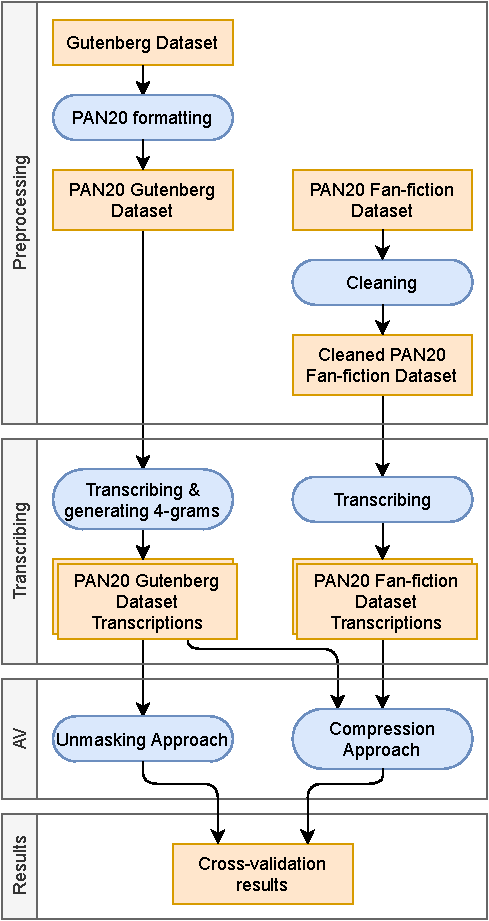
\includegraphics[width=0.6\textwidth]{figures/process}
  \caption{Experimental setup}
  \label{fig:process}
\end{figure}

\section{Datasets}
We use learning-based classification algorithms.
This means, given a set of rules, they try to induce the underlying patterns of a training set.
The resulting patterns are then used to classify unseen entities of a test set.
To train and test our algorithms we use two datasets, each consisting of labeled text pairs.
A pair has the label $True$ if both texts were authored by the same person and $False$ if not.\\\\
% PAN20 fan-fiction
First, we will use the small official dataset from the PAN2020 task on Authorship Verification from \cite{bevendorff2020overview}.
This allows us to compare our results to the other methods submitted.
It consists of 52.601 text pairs collected from the fanfiction website \url{fanfiction.net}.
The dataset file is formatted in the PAN20 format with each line containing a json object with the text pair, an ID, and optionally some additional information such as the corresponding fandoms\footnote{The franchise a fanfiction text belongs to. It can be seen as the topical domain of the text.}.
In contrast, the large official dataset contains 256.000 samples.
This is roughly five (4.86) times as many samples as the small data set.
Efforts have been made to maximally optimize the methods used, but due to some implementation details, the utilization of this dataset is infeasible for now.\\
% Gutenberg
We source the second dataset from \cite{stein2019unbiasedGutenbergCorpus}.
It presents a dataset containing science fiction and adventure texts from the 19th and 20th century, compiled from books from Project Gutenberg\footnote{\url{https://www.gutenberg.org/}}.
As discussed earlier, the aim of this dataset is to reduce common biases in data sets for Authorship Verification.
This makes it a good candidate for evaluating new authorship verifiers.
With only 262 text pairs, it is much smaller than the first dataset used.
% It is well suited for the much slower Unmasking algorithm, but might lead to overfitting.
To mitigate overfitting, we use out-of-fold cross-validation to evaluate the models instead of a standard train-test-split method.
This dataset is in the old PAN format\footnote{\textcolor{violet}{TBD: Used from PANXX to PANXX}} and is converted to the new PAN20 format for standardization\footnote{The code for the conversion is available at \url{https://github.com/torond/NAACL-19}}.\\

% Transcribing
% Repeat that the transcriptions are used as inputs
We use a range of open-source libraries to transcribe the datasets.
First, we transcribe a given text to IPA using g2pE introduced by \cite{kyubyong2019g2pE}.
Then we use the resulting transcription to generate the broader sound class transcriptions using the Cross-Linguistic Transcription Systems project by \cite{list2018cltsIntro}.
CLTS serves as a mapping between different transcription and sound class systems.
Given a list of IPA transcribed phonemes, they can be mapped to a range of different transcription systems.\\
To begin with, g2pE expands numbers and currency symbols (e.g.,\ '\$400' -> 'four hundred dollars').
It uses part-of-speech tags to find the correct pronunciations for heteronyms and then looks up pronunciations in the Carnegie Mellon University Pronouncing Dictionary\footnote{\url{http://www.speech.cs.cmu.edu/cgi-bin/cmudict/}}.
For out-of-vocabulary words it employs a neural net model to predict their correct pronunciations.\\
We use this algorithm, because it produces IPA representations, segmented into phonemes.
\cite{list2018sequence} recommends using these segmented IPA representations.
Words in IPA can contain arbitrary supra-segmental letters, and it is hard to segment these words into phonemes after transcribing.
Transcribing, for example, the word "make" to IPA results in \textipa{[meIk]}.
In contrast to other algorithms, g2pE produces the correct segmentation \textipa{[m eI k]}.
Using CLTS to convert this to the $Dolgo$ system we correctly get "MVK".
If we were, for example, to naively segment \textipa{[meIk]} to \textipa{[m e I k]} by interpreting each IPA symbol as a phoneme, we would incorrectly get "MVVK" as a result for the $Dolgo$ system.\\
As Soundex, Refined Soundex and Metaphone work on verbatim text directly, we create those transcriptions with a different library, pyphonetics\footnote{\url{https://github.com/Lilykos/pyphonetics}}.
The source code in this library is based \textcolor{teal}{(on Talisman.js which itself is based)} on the Apache commons codec\footnote{\url{http://commons.apache.org/proper/commons-codec/userguide.html}}.
Punctuation and stop word removal, as well as lemmatization is done with spaCy\footnote{\url{https://spacy.io/}} for speed and robustness.
The source code for transcribing PAN20 datasets is available on GitHub\footnote{\url{https://github.com/torond/ba-util}}.


% 1.2 Compression Approach
\section{Compression Approach}
The first approach, introduced in PAN2020 and based on \cite{teahan2003compression}, uses a text compression method to determine the chance that two texts were written by the same author.
The compression of a text can be seen as encoding said text with a given encoding.
Thus, as discussed in \cite{brown1992upperBoundEntropy}, text compression can be used to estimate an upper bound to the entropy, i.e. the amount of information of characters in English text.
More specific, by using the compression model of some text A, the cross-entropy of encoding a text B with this model can be calculated.
This approach uses the Prediction by Partial Matching (PPM) model, a standard model for lossless text compression, first introduced by \cite{cleary1984PPM}.
During training, for each pair, the PPM of the first text is used to encode the second text and vice-versa.
In this process, the cross-entropy of the first to the second text can be calculated and vice-versa.
In other words, if the compression of one text with the compression model of the second text works well, the chance that both are written by the same author can be considered high.
The source code used is based on a reimplementation of the Authorship Attribution approach from \cite{teahan2003compression} as part of a reproducibility study in \cite{potthast2016reimplementation}.
An adaption for Authorship Verification stems from PAN20\footnote{\url{https://github.com/pan-webis-de/pan-code/tree/master/clef20/authorship-verification}}.
The source code extending the algorithm to use phonetic features is available on GitHub\footnote{\url{https://github.com/torond/teahan03-phonetic}}.
% Add figure, only showing cross-validation side!

% 1.3 Unmasking Approach
\section{Unmasking Approach}
% Intro: Embedding in context of related work (at the time), more complex but now baseline
% Invented by Koppel & Schler, cite paper
Unmasking was first introduced by \cite{koppel2004unmasking} in 2004.
% Main idea 1-2 sentences: Why is it called Unmasking? feature removal -> degradation
In short, it exploits the degradation of classifier accuracy when removing distinguishing features.
It turns out that removing those features iteratively leads to a faster degradation on text pairs by one author than on those by different authors.
Thus, the algorithm "unmasks" the text pairs and thereby reveals the information needed for classification.\\

% Formal definiton & explanation: unmasking step
This approach comprises two steps: First, a cross-validation method is employed to create the accuracy degradation curves for all training samples.
Secondly, a meta-classifier is trained on the resulting curves to differentiate between same-author and different-author curves.\\
For a given pair, the texts are seen to be created by two generative processes $p_1$ and $p_2$.
To compute a curve for a pair, both texts are chunked into parts longer then 500 words without splitting paragraphs.
The 250 words with highest average frequencies in the two texts are used as features.
\textcolor{violet}{TBD: Note bag-of-words approach}
In a 10-fold cross-validation linear SVM models are trained to classify if a chunk belongs to $p_1$ or $p_2$.
The resulting accuracy is noted and the three most influential positive and negative features are removed from the feature set \textcolor{teal}{(Is influential the right word here?)}.
The cross-validation and feature removal are repeated until there are no features left.\\
% meta-learning step
The set of curves is then used to train a meta-classifier linear SVM model.
\textcolor{teal}{Note: Rearrange the following sentences to only cite \cite{bevendorff2019unmaskingShortTexts} once.}
As brought to the point by \cite{bevendorff2019unmaskingShortTexts}, features used are "the curve points, the curves' point-wise first- and second-order derivatives, and the derivatives sorted by steepest point-wise drop" \textcolor{teal}{(Should this be paraphrased rather then quoted?)}.\\
% Adaptation for short texts by Bevendorff et al., how is this different? Which features are actually being used?
Unmasking is one of the most robust Authorship Verification algorithms \textcolor{teal}{(\cite{bevendorff2019unmaskingShortTexts})}.
But as it requires sufficient chunks of no less than 500 words length, it is only applicable for book-length texts.
To counter this, \cite{bevendorff2019unmaskingShortTexts} generalizes the algorithm to accommodate for short texts.
Chunks are generated by oversampling the bag-of-words pool of a given text.
Words from this pool are picked randomly without replacement until a length of 700 words is reached and the pool is reset afterwards.
In total, 30 chunks are generated, which are then used for curve generation as above, with the only exception that the five most positive and negative features are removed instead of only three.
As this approach introduces a significant amount of variance in the resulting curves, the unmasking step is repeated three times and the curves are averaged.
This time, the meta-classifier uses the curves' "central-difference gradients (first- and second-order), as well as their gradients sorted by magnitude" \textcolor{teal}{(\cite{bevendorff2019unmaskingShortTexts})}.
\cite{bevendorff2019unmaskingShortTexts} also supplies an implementation of the generalized unmasking algorithm which is used as the basis for our research\footnote{\url{https://github.com/webis-de/unmasking}}.\\
\textcolor{violet}{TBD: Explain that we'll use transcriptions with bag-of-words first, then $Dolgo$ with n-grams.}
%We conduct two experiments using the unmasking algorithm.
%First, we simply used phonetic transcriptions of text pairs as the input to the unmasking algorithm.
%Secondly, we use the features $features_{clever}$ (change notation) instead of the averagely most frequent words.
Note that we only use the Gutenberg dataset for unmasking, as processing the fanfiction dataset would for each of the transcriptions would take multiple weeks.
%We suspect that the differences would not be significant. (Can I phrase that like this??)
We added an out-of-fold cross-validation functionality to the unmasking framework to extract as much information as possible from the much smaller Gutenberg dataset.
The results are then compared to results obtained from verbatim text.
%(Maybe add more code details! What else was added etc.)

%Notes (Koppel and Schler 2004):
%AV as described in the paper is Authorship Attribution -> Goes on to reformulate: AV's question is whether a pair of text sets were created by the same process (author) or different processes.
%-> How does this extend to sets when there's more than 1 author in the "investigated" set?
%-> It sounds like the set of same-author texts must have one author.
%-> Also in paper we have 2 sets of texts, in PAN AV we have a list of pairs. Is this the same?
%Determines "depth of difference" between two sets of texts

%\section{Methods using supra-segmental features}
%% Time Series Modelling in the Analysis of Homeric Verse, Pawłowski 2010
%Manual annotation of long / short syllables and stress / no-stress syllables (p.86).
%ARIMA method for time series modelling.\\
%Rhythmical series are easier to model -> goodness of fit ~ rhythmicity
%
%
%"All the suprasegmental features are characterized by the fact that they must be described in relation to other items in the same utterance.
%It is the relative values of pitch, length, or degree of stress of an item that are significant.
%... The absolute values are never linguistically important.
%But they do, of course, convey information about the speaker's age, sex, emotional state, and attitude toward the topic under discussion."\cite{ladefoged2014courseInPhonetics}

% http://udel.edu/~dlarsen/ling101/slides/Suprasegmentalshandout.pdf
% english has non-distinctive length differences.
% p.15 In English, stress is sometime non-predictable, sometimes predictable.